\newpage
\section{Feasibility}
Una volta creato il dataframe contenente la matrice delle distanze, siamo pronti per l'avvio del \emph{Feasibility test}. Questa fase prende in input la precedentemente citata matrice con un determinato campo che sarà il nostro \emph{RHS}. Ovviamente, i restanti campi, formeranno il nostro \emph{LHS}.
\begin{table}[H]
	\centering
	\begin{tabular}{l l l l l l l l}
		height & weight & shoe{\_}size & age \\
		\hline
		175 & 70 & 40 & 30\\
		175 & 75 & 39 & 41\\
		175 & 69 & 40 & 33\\
		176 & 71 & 40 & 35\\
		178 & 81 & 41 & 27\\
		169 & 73 & 38 & 49\\
		170 & 65 & 39 & 30\\
	\end{tabular}
	\caption{Dataset di esempio.}
	\label{tab:Dataset_di_esempio}
\end{table}
\begin{table}[H]
	\centering
	\begin{tabular}{l l l l l l l l}
		height & weight & shoe{\_}size & age & TuplePairID\\
		\hline
		0 & 5 & 1 & 11 & 0-1\\
		0 & 6 & 1 & 8 & 1-2\\
		\vdots & \vdots &  \vdots &  \vdots &  \vdots \\
		1 & 8 & 1 & 19 & 5-6\\
	\end{tabular}
	\caption{Esempio matrice delle distanze}
	\label{tab:Esempio_DM}
\end{table}
Nel seguente pseudocodice diamo una occhiata su quello che dovrebbe effettuare il nostro algoritmo durante la fase corrente:\\
\begin{figure}[H]
	\centering
	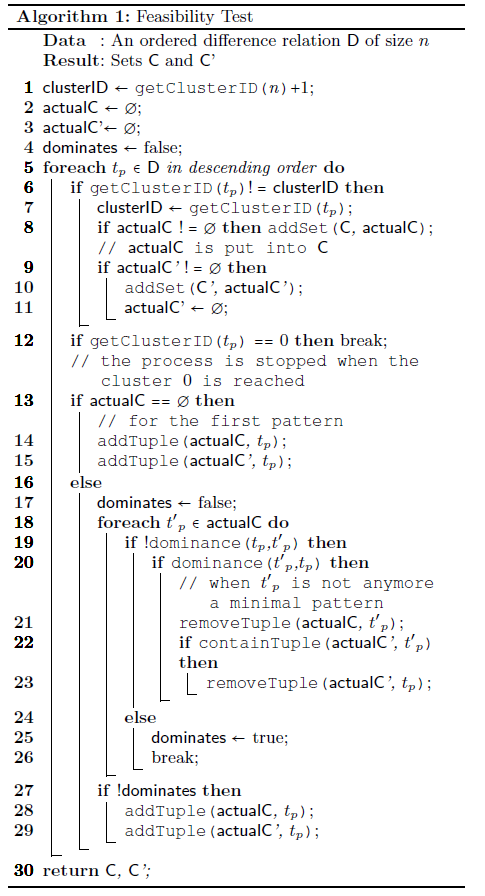
\includegraphics[scale = 0.7]{Immagini/Feasibility.png}
	\caption{Pseudocodice Feasibility Test}
	\label{fig:Pseudocodice Feasibility Test}
\end{figure}
Come detto nella fase di creazione della matrice delle distanze, tale matrice è stata ordinata per il valore dell'\emph{RHS} e successivamente sono stati raggruppati i pattern con valori uguali di tale campo(\emph{Cluster})\footnote{Per questo algoritmo ci riferiremo a ClusterN come il gruppo di pattern aventi N come valore di RHS }.
Lo scopo di questa fase è l'ottenimento di insiemi contenenti pattern che superino il test di Feasibility, tali insiemi saranno costruiti uno per ogni valore differente di RHS.
Come si evince dallo pseudocodice l'analisi ha inizio con il clusterN con N di valore massimo.
Per questo caso l'insieme viene inizializzato con l'ultima riga trovata, essendo l'insieme ancora vuoto.
L'analisi per questo cluster proseguirà con le altre righe, esse saranno inserite nell'insieme in costruzione corrente solo se non dominano quelle già presenti. La verifica della dominanza(concetto espletato nell'introduzione), però, è effettuata non solo dalla riga da inserire verso quelle già presenti, tale controllo viene effettuato anche dai pattern esistenti verso la riga che vuole "entrare" nell'insieme. Se il risultato della dominanza rileva che un pattern nell'insieme \emph{domina} la riga in entrata, allora questo viene rimosso.
Il duplice controllo ci garantirà che in uno stesso cluster non ci siano pattern che dominano altri.
Una volta finita l'analisi di un cluster, l'algoritmo avrà l'insieme corrispondente e sarà pronto ad analizzare quello successivo. Per effettuare questo cambio, l'insieme corrispondente verrà inizializzato con i pattern facente parte dell'insieme ottenuto in precedenza.
Questa analisi verrà conclusa o con la fine dei cluster disponibili oppure quando si giunge ad un valore di \emph{RHS uguale a 0}.
Infine, avremo ottenuto un insieme di pattern per ogni cluster, tali insiemi sono definiti \textbf{insiemiC}.
A questo punto, con il nostro output, potremo procedere verso le fasi di \emph{Minimality e RFD Generation}.
